\documentclass[11pt,a4paper,oneside]{article}

\usepackage[english,russian]{babel}
\usepackage[T2A]{fontenc}
\usepackage[utf8]{inputenc}
\usepackage{graphicx}
\usepackage{expdlist}
\usepackage{mfpic}
\usepackage{amsmath}
\usepackage{amssymb}
\usepackage{comment}
\usepackage{listings}
\usepackage{epigraph}
\usepackage{url}

\DeclareMathOperator{\nott}{not}

\begin{document}

\renewcommand{\t}[1]{\mbox{\texttt{#1}}}
\newcommand{\s}[1]{\mbox{``\t{#1}''}}
\newcommand{\eps}{\varepsilon}
\renewcommand{\phi}{\varphi}
\newcommand{\plainhat}{{\char 94}}

\newcommand{\Z}{\mathbb{Z}}
\newcommand{\w}[1]{``\t{#1}''}

\author{Андрей Комаров}
\title{Лабораторная работа \No2. Ручное построение нисходящих синтаксических анализаторов}
\date{11 апреля 2013 года}
\maketitle

\section{Разработка грамматики}

\subsection{Задание}
Описание переменных в Паскале.

\subsection{Построение грамматики}
\begin{tabular}{ r c l }
    $S$ & $\to$ & $\mathrm{var}\, D$ \\
    $D$ & $\to$ & $E\, D\, |\, \varepsilon$ \\
    $E$ & $\to$ & $\mathrm{n}\, I\, \mathrm{:\, n\, ;}$ \\
    $I$ & $\to$ & $\mathrm{,\, n}\, I\, |\, \varepsilon$ \\
\end{tabular}

\begin{center}
    \begin{tabular}{ | l | l | }
        \hline
        \textbf{Нетерминал} & \textbf{Описание} \\
        \hline
        $S$ & Начальный нетерминал. \\
        \hline
        $D$ & Список определений. \\
        \hline
        $E$ & Одно определение. \\
        \hline
        $I$ & Список переменных. \\
        \hline
    \end{tabular}
\end{center}

В грамматике нет левой рекурсии или правого ветвления. 


\section{Построение лексического анализатора}

В нашей грамматике четыре терминала: <<:>> (двоеточие), <<;>> (точка с запятой),
<<,>> (запятая) и <<n>> (идентификатор).

\begin{verbatim}
data Lexem 
    = Colon
    | Semicolon
    | Comma
    | Name String deriving (Eq, Show, Read)
\end{verbatim}

\begin{tabular}{| l | c |}
    \hline
    \textbf{Терминал} & \textbf{Токен} \\
    \hline
    : & \verb+Colon+ \\
    \hline
    ; & \verb+Semicolon+ \\
    \hline
    , & \verb+Comma+ \\
    \hline
    ident & \verb+Name+ \\
    \hline
\end{tabular}


\section{Построение синтаксического анализатора}

Построим множества \textbf{FIRST} и \textbf{FOLLOW} для нетерминалов.

% S -> "var" D
% D -> ED | eps
% E -> n I : n ;
% I -> , n I | eps

\begin{tabular}{| l | l | l |}
    \hline
    \textbf{Нетерминал} & \textbf{FIRST} & \textbf{FOLLOW} \\
    \hline
    $S$ & n(<<var>>) & n, \$ \\
    \hline
    $D$ & n, $\varepsilon$ & n, \$ \\
    \hline
    $E$ & n & n, \$ \\
    \hline
    $I$ & n, $\varepsilon$ & : \\
    \hline
\end{tabular}
\\
Структуры для хранения дерева полностью повторяют грамматику:

\begin{verbatim}
data SNode = SNode DNode
data DNode = DNode ENode DNode | DEps
data ENode = ENode String INode String
data INode = INode String INode | IEps
\end{verbatim}



\section{Набор тестов + визуализация}
\subsection{Тест \No1}

\texttt{var a : int;}

Ожидается успех

Успех! 

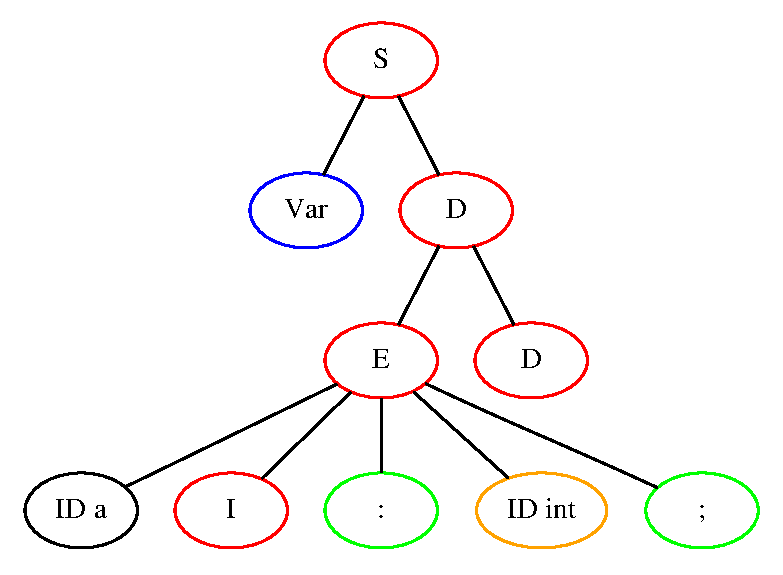
\includegraphics[width=\textwidth]{test1.eps}

\subsection{Тест \No2}

\texttt{vbr b : int;}

Ожидается провал

Ошибка: \texttt{Expected Name "var", found Name "vbr"}

\subsection{Тест \No3}

\texttt{var a, b : int;}

Ожидается успех

Успех! 

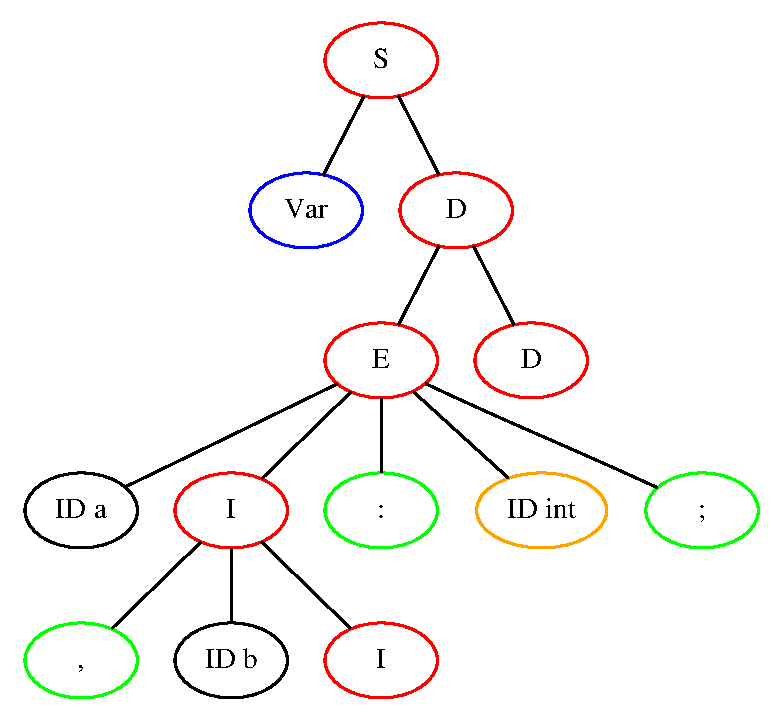
\includegraphics[width=\textwidth]{test3.eps}

\subsection{Тест \No4}

\texttt{var a, b :: int;}

Ожидается провал

Ошибка: \texttt{Expected Type name, found Colon}

\subsection{Тест \No5}

\texttt{var a, b : int; c : int;}

Ожидается успех

Успех! 

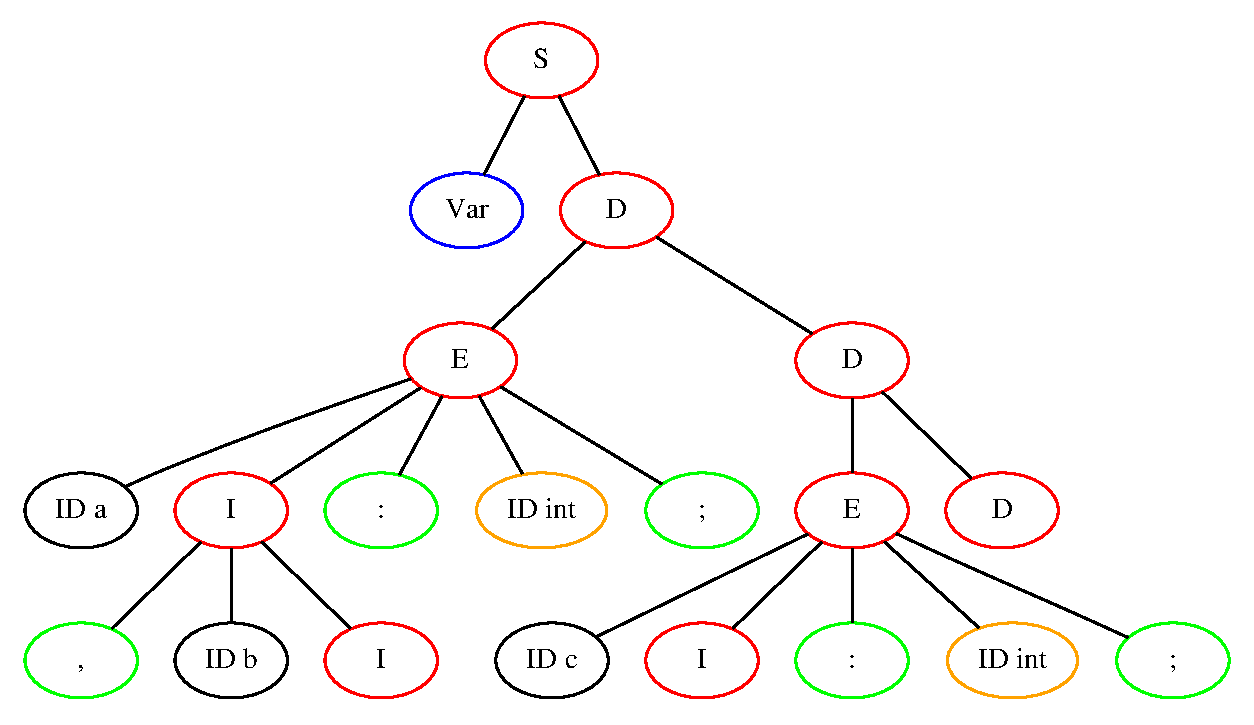
\includegraphics[width=\textwidth]{test5.eps}

\subsection{Тест \No6}

\texttt{var a, b : int; c, d : int;}

Ожидается успех

Успех! 

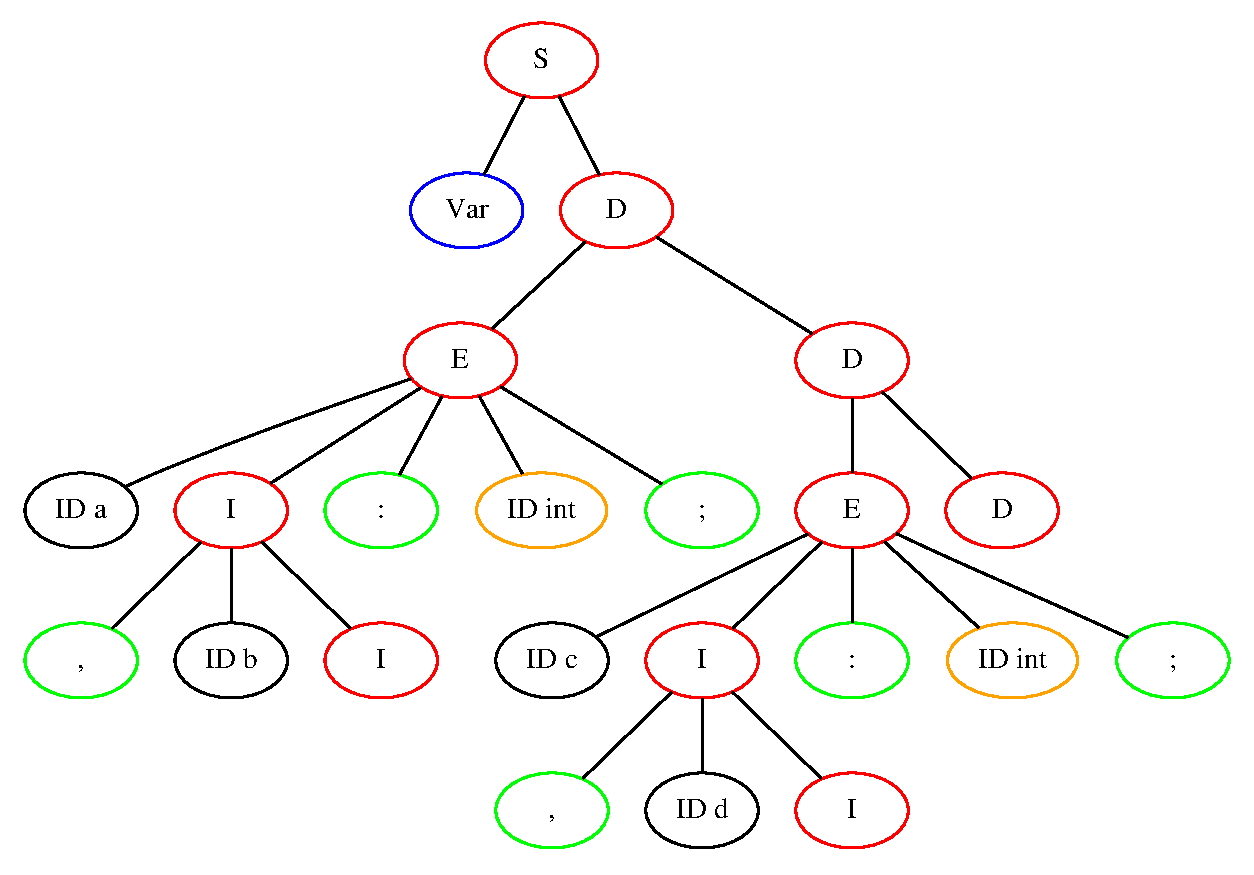
\includegraphics[width=\textwidth]{test6.eps}

\subsection{Тест \No7}

\texttt{var a,, b : int;}

Ожидается провал

Ошибка: \texttt{Expected Variable name, found Comma}

\subsection{Тест \No8}

\texttt{var a, b, c : int;;}

Ожидается провал

Ошибка: \texttt{Expected Variable name, found Semicolon}

\subsection{Тест \No9}

\texttt{var a : int}

Ожидается провал

Ошибка: \texttt{Expected Semicolon, found EOLN}

\subsection{Тест \No10}

\texttt{v a r a : int}

Ожидается провал

Ошибка: \texttt{Expected Name "var", found Name "v"}

\subsection{Тест \No11}

\texttt{     var a : int}

Ожидается провал

Ошибка: \texttt{Expected Semicolon, found EOLN}

\subsection{Тест \No12}

\texttt{var}

Ожидается успех

Успех! 

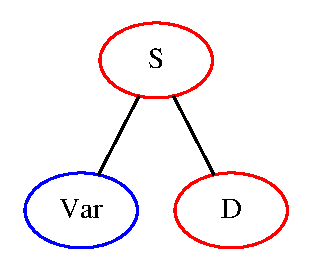
\includegraphics[width=\textwidth]{test12.eps}

\subsection{Тест \No13}

\texttt{var ololo : a;}

Ожидается успех

Успех! 

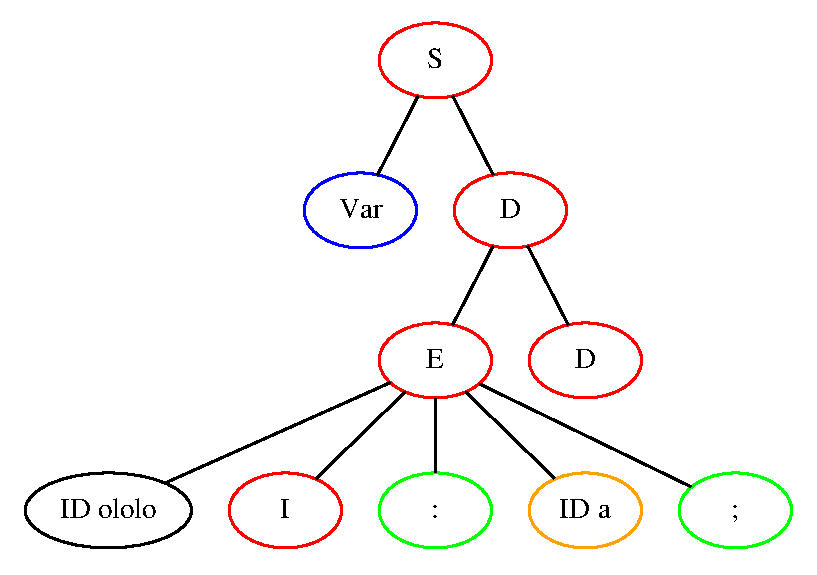
\includegraphics[width=\textwidth]{test13.eps}

\subsection{Тест \No14}

\texttt{var ololo, tata, asda, asdf : asldfa; asdf, asdfas,f,asdf,asdf : double;a,b,c,d,e,f,g:bool;}

Ожидается успех

Успех! 

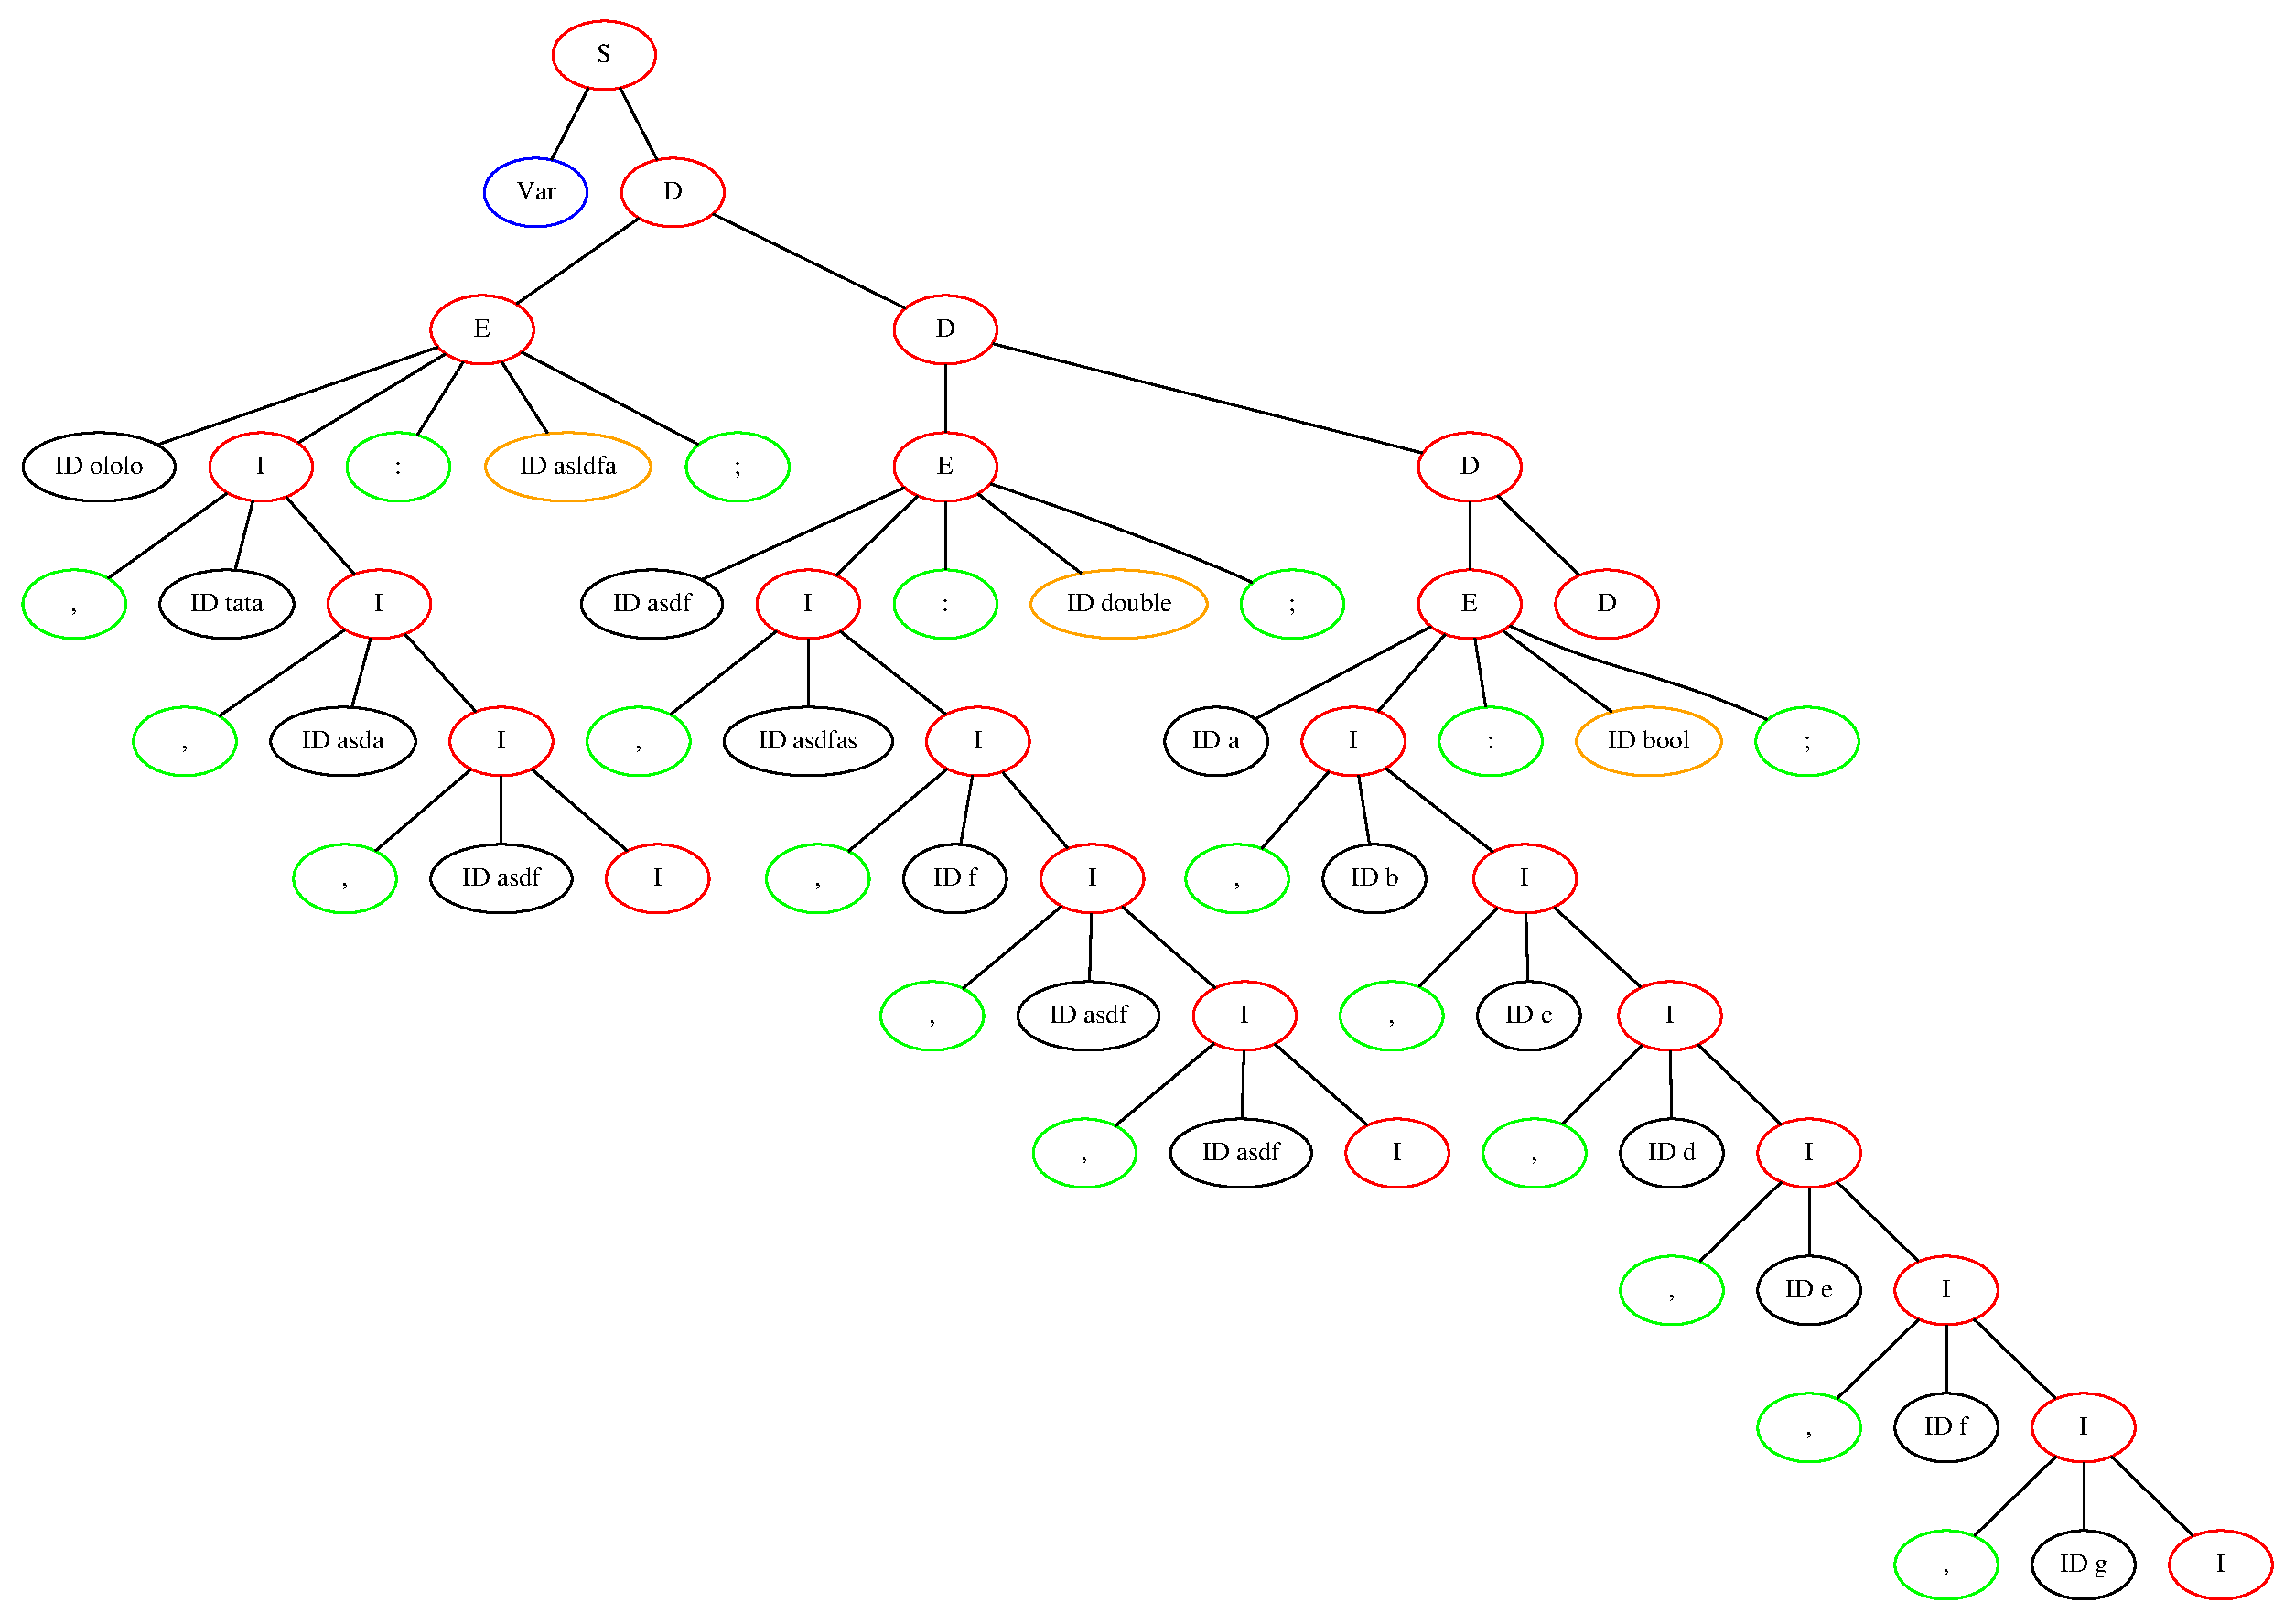
\includegraphics[width=\textwidth]{test14.eps}



\end{document}
